\documentclass{scrreprt}

\usepackage{listings}
\usepackage{underscore}
\usepackage{graphicx,subfigure}

\usepackage[bookmarks=true]{hyperref}
\usepackage[utf8]{inputenc}
\usepackage[english]{babel}
\usepackage{hyperref}

\hypersetup{
    bookmarks=false,    % show bookmarks bar?
    pdftitle={Upstack Hackathon 2018 Kalimotxo App Product Plan},    % title
    pdfauthor={Bogdan Lupu, Hasan Shingieti, Mauricio De La Quintana},                     % author
    pdfsubject={},                        % subject of the document
    pdfkeywords={}, % list of keywords
    colorlinks=true,       % false: boxed links; true: colored links
    linkcolor=blue,       % color of internal links
    citecolor=black,       % color of links to bibliography
    filecolor=black,        % color of file links
    urlcolor=purple,        % color of external links
    linktoc=page            % only page is linked
}%
\def\myversion{1.0}
\date{}
%\title 
\usepackage{hyperref}
\begin{document}

\begin{flushright}
    \rule{16cm}{5pt}\vskip1cm
    \begin{bfseries}
        \Huge{Product Plan}\\
        \vspace{1.9cm}
        Kalimotxo - Bartender Rating App\\
        \vspace{1.9cm}
        \LARGE{Version \myversion}\\
        \vspace{1.9cm}
        Upstack Hackathon 2018 Team 7\\
        \vspace{1.9cm}
        October 27, 2018
    \end{bfseries}
\end{flushright}

\tableofcontents


%\chapter*{Revision History}
%
%\begin{center}
%    \begin{tabular}{|c|c|c|c|}
%        \hline
%	    Name & Date & Reason For Changes & Version\\
%        \hline
%	    21 & 22 & 23 & 24\\
%        \hline
%	    31 & 32 & 33 & 34\\
%        \hline
%    \end{tabular}
%\end{center}

\chapter{Introduction}

\section{Purpose}
The purpose of this document is to build an online system for bartender rating app.
This app aims make the relationship between customers and bartenders more personal.
The name of the app will be \hyperlink{https://www.supercall.com/recipe/kalimotxo-drink-recipe}{Kalimotxo} and is pronounced in spanish
\hyperlink{https://forvo.com/word/kalimotxo/}{Calimocho}.

\section{Intended Audience}
This document is intended for business owners, investors, developers, and designers so they can have a better understanding as to the goal of the application and its features. The people and teams involved in the creation, design, and implementation of the application have a wide scope of knowledge of the market needs, functional requirements, and underlying technology to create a modern web app. The sections in this document are not technical and are intended to provide an overview, in common terms, of what the application is and the features it will implement.

\section{Project Scope}
The application is designed to enhance the relationship between customers and servers by providing a platform for feedback based on individual service. Users who use and engage with others in the application will benefit from social feedback and receive rewards for their participation and positive performance. The goal of the application is to allow people - local residents, business travelers, and fun-seekers - to find top service in their area. The information gathered by user input will provide valuable insight into customer sentiment on an individual level which allows for better performance and increased revenue for business owners, and, in turn, higher engagement within the application.

\chapter{Overall Description}

% \section{Product Perspective}
% $<$Describe the context and origin of the product being specified in this SRS.
% For example, state whether this product is a follow-on member of a product
% family, a replacement for certain existing systems, or a new, self-contained
% product. If the SRS defines a component of a larger system, relate the
% requirements of the larger system to the functionality of this software and
% identify interfaces between the two. A simple diagram that shows the major
% components of the overall system, subsystem interconnections, and external
% interfaces can be helpful.$>$

% \section{Product Functions}
% $<$Summarize the major functions the product must perform or must let the user
% perform. Details will be provided in Section 3, so only a high level summary
% (such as a bullet list) is needed here. Organize the functions to make them
% understandable to any reader of the SRS. A picture of the major groups of
% related requirements and how they relate, such as a top level data flow diagram
% or object class diagram, is often effective.$>$

% \section{User Classes and Characteristics}
% $<$Identify the various user classes that you anticipate will use this product.
% User classes may be differentiated based on frequency of use, subset of product
% functions used, technical expertise, security or privilege levels, educational
% level, or experience. Describe the pertinent characteristics of each user class.
% Certain requirements may pertain only to certain user classes. Distinguish the
% most important user classes for this product from those who are less important
% to satisfy.$>$

\section{Operating Environment}
The application will be available in all major browsers.

\section{Design and Implementation Constraints}
\subsection{Technology Stack}
Backend:
\begin{itemize}
    \item Node.js
    \item Express.js
    \item Firebase
\end{itemize}
Frontend:
\begin{itemize}
    \item Angular 2+
    \item Angular Material
\end{itemize}
\newpage
\subsection{Application Flow}
\begin{figure}[h]
	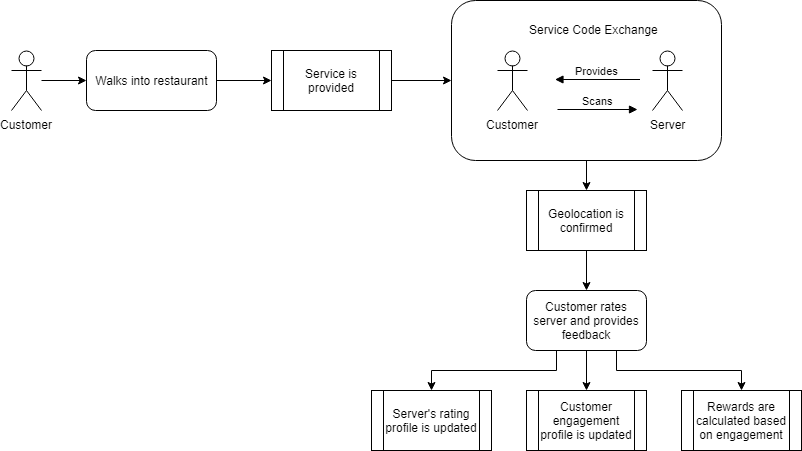
\includegraphics[width=\textwidth]{uml/process-flow-diagram}
	\centering
\end{figure}

% \section{User Documentation}
% $<$List the user documentation components (such as user manuals, on-line help,
% and tutorials) that will be delivered along with the software. Identify any
% known user documentation delivery formats or standards.$>$
% \section{Assumptions and Dependencies}

% $<$List any assumed factors (as opposed to known facts) that could affect the
% requirements stated in the SRS. These could include third-party or commercial
% components that you plan to use, issues around the development or operating
% environment, or constraints. The project could be affected if these assumptions
% are incorrect, are not shared, or change. Also identify any dependencies the
% project has on external factors, such as software components that you intend to
% reuse from another project, unless they are already documented elsewhere (for
% example, in the vision and scope document or the project plan).$>$


% \chapter{External Interface Requirements}

% \section{User Interfaces}
% $<$Describe the logical characteristics of each interface between the software
% product and the users. This may include sample screen images, any GUI standards
% or product family style guides that are to be followed, screen layout
% constraints, standard buttons and functions (e.g., help) that will appear on
% every screen, keyboard shortcuts, error message display standards, and so on.
% Define the software components for which a user interface is needed. Details of
% the user interface design should be documented in a separate user interface
% specification.$>$

% \section{Hardware Interfaces}
% $<$Describe the logical and physical characteristics of each interface between
% the software product and the hardware components of the system. This may include
% the supported device types, the nature of the data and control interactions
% between the software and the hardware, and communication protocols to be
% used.$>$

% \section{Software Interfaces}
% $<$Describe the connections between this product and other specific software
% components (name and version), including databases, operating systems, tools,
% libraries, and integrated commercial components. Identify the data items or
% messages coming into the system and going out and describe the purpose of each.
% Describe the services needed and the nature of communications. Refer to
% documents that describe detailed application programming interface protocols.
% Identify data that will be shared across software components. If the data
% sharing mechanism must be implemented in a specific way (for example, use of a
% global data area in a multitasking operating system), specify this as an
% implementation constraint.$>$

% \section{Communications Interfaces}
% $<$Describe the requirements associated with any communications functions
% required by this product, including e-mail, web browser, network server
% communications protocols, electronic forms, and so on. Define any pertinent
% message formatting. Identify any communication standards that will be used, such
% as FTP or HTTP. Specify any communication security or encryption issues, data
% transfer rates, and synchronization mechanisms.$>$


\chapter{System Features}
The system must provide,at a minimum, the following functions
in accordance with the other requirements described within
this SRS document.
% $<$This template illustrates organizing the functional requirements for the
% product by system features, the major services provided by the product. You may
% prefer to organize this section by use case, mode of operation, user class,
% object class, functional hierarchy, or combinations of these, whatever makes the
% most logical sense for your product.$>$

\section{Register System}
The system should have a register system for the user.

% \subsection{Description and Priority}
% $<$Provide a short description of the feature and indicate whether it is of
% High, Medium, or Low priority. You could also include specific priority
% component ratings, such as benefit, penalty, cost, and risk (each rated on a
% relative scale from a low of 1 to a high of 9).$>$

% \subsection{Stimulus/Response Sequences}
% $<$List the sequences of user actions and system responses that stimulate the
% behavior defined for this feature. These will correspond to the dialog elements
% associated with use cases.$>$

% \subsection{Functional Requirements}
% $<$Itemize the detailed functional requirements associated with this feature.
% These are the software capabilities that must be present in order for the user
% to carry out the services provided by the feature, or to execute the use case.
% Include how the product should respond to anticipated error conditions or
% invalid inputs. Requirements should be concise, complete, unambiguous,
% verifiable, and necessary. Use “TBD” as a placeholder to indicate when necessary
% information is not yet available.$>$

% $<$Each requirement should be uniquely identified with a sequence number or a
% meaningful tag of some kind.$>$
% \begin{enumerate}
%     \item REQ-1:
%     \item REQ-2:
% \end{enumerate}

\section{Authorization and Authentication System}
The system should have a login system for the user and based on
their roles they will access different views in the app.
\begin{itemize}
    \item As a customer i will have the capability to leave comments and readings.
    \item As a bartender i will have access to my profile.
    \item As a business unit i will have access to my dashboard.
\end{itemize}

\section{QR Code Generator}
As a bartender after you are registered in the app you will receive a unique qrcode.
The bartender can print the qrcode or present from the phone the qrcode to the customer.

\section{QR Code Scanner}
As a user i need to be able to scan the qrcode provided by the bartender.

\section{User Profile}
\begin{itemize}
    \item As a user, i need a profile view where I'm able to change my profile picture add a description.
    \item As a bartender i need a view of all my reviews received form customers.
    \item As a business unit i need a profile view where I`m able to change my addresses
\end{itemize}

\section{Customer rating}
As a user after I scanned the qr code from the bartender:
\begin{itemize}
    \item I need a view with the bartender profile and rating.
    \item I need the capability to add a comment and rating for a bartender
\end{itemize}

\section{Hall of Fame}
As a non login in user i have access to the bartenders Hall of Fame.

\section{Heat Map}
As a login in customer i have access to a heat map where i can see the most crowded near me.

\section{Business Unit Premium Dashboard}
As a business owner i have a dashboard to see premium features such as employee performance, frequent customers, and available rewards

\section{Functional Requirements}
The application should be mobile friendly.

\section{System Data}
\begin{enumerate}
	\item Customers
	\begin{itemize}
		\item User ID
		\item First name
		\item Last name
		\item Email
		\item Score
		\item Location
	\end{itemize}
	\item Servers
	\begin{itemize}
		\item User ID
		\item First name
		\item Last name
		\item Email
		\item Overall Rating
		\item Service Code
		\item Location
	\end{itemize}
	\item Ratings
	\begin{itemize}
		\item Server ID
		\item Restaurant ID
		\item Comment
		\item Rating
	\end{itemize}
	\item Restaurants
	\begin{itemize}
		\item Name
		\item Owner
		\item Restaurant ID
		\item Rewards
	\end{itemize}
\end{enumerate}

\chapter{User Interface}

\begin{figure}[!htb]
    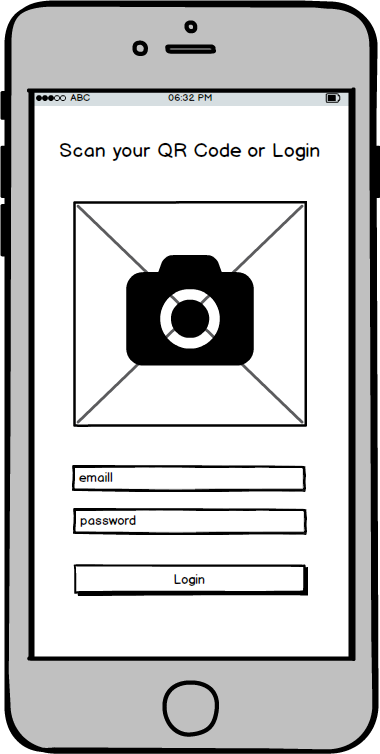
\includegraphics[width=6cm, height=12cm]{mockups/Login}
    \centering
    \caption{Login}
\end{figure}

\begin{figure}[!htb]
    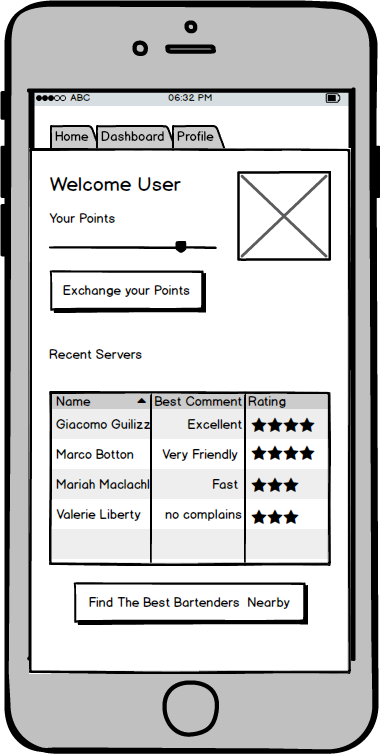
\includegraphics[width=6cm, height=12cm]{mockups/Home}
    \centering
    \caption{Home}
\end{figure}

\begin{figure}[!htb]
    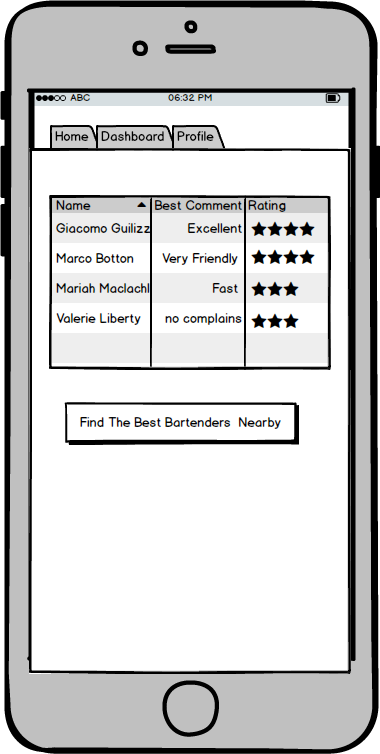
\includegraphics[width=6cm, height=12cm]{mockups/Dashboard}
    \centering
    \caption{Dashboard}
\end{figure}

\begin{figure}[!htb]
    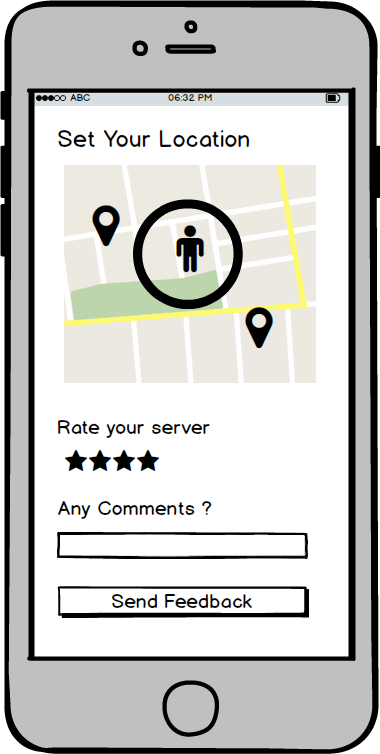
\includegraphics[width=6cm, height=12cm]{mockups/Feedback}
    \centering
    \caption{Feedback}
\end{figure}

\end{document}